\section{Results}
\begin{figure}
  \centering%
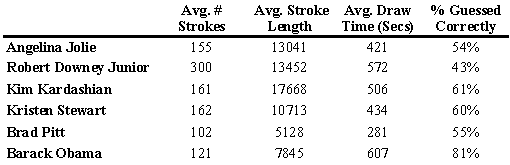
\includegraphics[height=1.1in]{./figures/daf-stats-cropped.pdf}
  \caption{Celebrity drawing statistics for 611 hand-picked drawings from the first four days after launch.}
  \label{fig:daf-stats}
\end{figure}



After smaller-scale trials, DrawAFriend was released publicly on January 8th, 2013. In 88 days there were 14,270 drawings. After the launch of DrawAFriend, our project proceeded in three phases. First we collected drawings for six celebrities to prime our initial correction vector field. Second we use the correction field to add an automatic stroke correction helper into the game. Lastly we crowd sourced the evaluation of our stroke corrector, by AB testing it within the game.

\subsection{DrawAFriend Correction Vector Field}
In order to integrate the correction vector field into the game, we needed to prime it with some initial drawings. In four days players had downloaded the game over 2000 times and created 6373 drawings. In that time, players had already spent approximately 10 full 24 hour days drawing. We used these drawings to create the correction vector field.


Players were given the option of drawing Facebook friends or one of an initial set of six celebrities: Robert Downey Jr., Angelina Jolie, Kim Kardashian, Barack Obama, Brad Pitt \cite{brad}, or Kristen Stewart. From the drawings generated in the first four days, we manually chose 611 celebrity drawings. For these drawings, players had made an attempt to accurately draw the eyes (the most intricate feature to draw). These 611 drawings were a little under 10\% of the dataset. The rest of the dataset mostly consisted of drawings that players had drawn quickly, resembling a person like scribble. While the rest of the dataset could be used for analysis, we did not train our correction vector field on it.  See Figure \ref{fig:daf-stats}  for statistics references these 611 drawings.

\begin{figure}
  \centering%
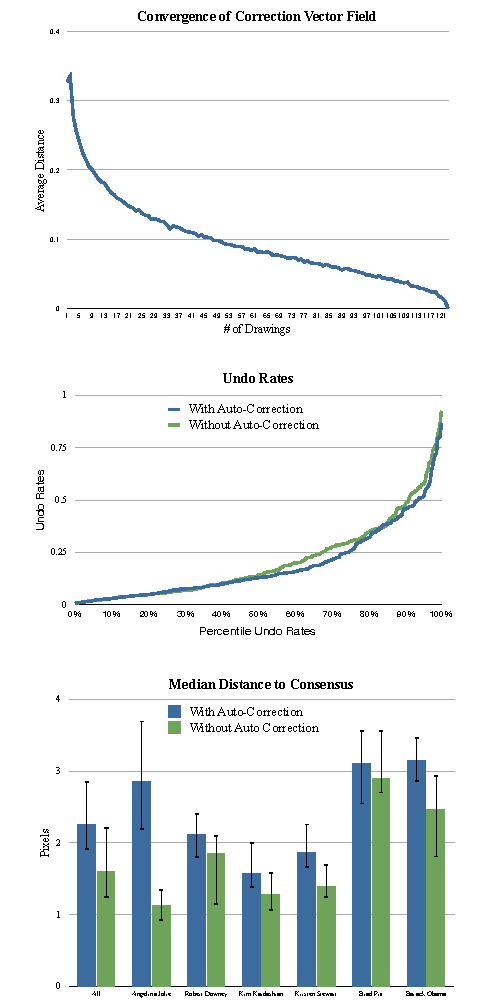
\includegraphics[width=3.5in]{./figures/userstudy/threeGraphs.pdf}
  \caption{(top) Convergence of the correction vector field as more images are added. Distance from convergence is measured as the mean Euclidean distance of the field from the full set of 131 images used.  (middle) Percentile undo rates for the auto-corrected and non auto-corrected drawings, sorted in ascending order. Note how the stroke auto correction decreases undo rates, particularly for more careful drawers. (bottom)The average distance between original uncorrected strokes and the consensus for each celebrity when auto-correction is on and off. Note that with auto-correction on users could be sloppier in their drawings that without auto-correction.}
  \label{fig:daf-three}
\end{figure}

We ran our modified mean shift algorithm on this initial dataset to create the correction vector fields shown in Figure \ref{fig:image-table}. Our MATLAB implementation took under 5 minutes for each celebrity.  The great majority of the time was spent in un-optimized nearest neighbor search. The correction vector field had the dimensions of 460x320. In Figure \ref{fig:daf-three} top we plot how our correction vector field converges for Brad Pitt, by calculating the vector field for a subset of the drawings. There appears to be an inflection point around 25 drawing, at which point the correction vector field would probably work well. However every drawing still improves the correction field, implying that after 130 drawings the correction vector field has not completely converged. We can also use the correction vector field to filter our drawings. Drawings whose points were on average 10 pixels away from the consensus were never actually portraits (most often they were simply someone writing out the celebrity's name). For the user study described below we used this filtering method to exclude non-portraits. 




\subsection {Drawing Enhancements}

We apply the correction vector field to interactively modify strokes during the drawing process. For every new stroke point added, a background thread is spun off to correct the new stroke. Once the thread completes if new points have accumulated another thread is immediately spun off. With no additional user interface elements to the existing DrawAFriend UI, we seamlessly add stroke auto-correction. As the user draws, strokes are subtly corrected at interactive rates on an iPhone 4. In general, the fact that corrections are being applied is almost invisible to the user. Instead, strokes appear where the user {\em intended} to draw.

%????Please see the \alex{Not sure how to reference the teaser on top} and the video for interactive examples.

We also applied the correction vector field retrospectively to improve the existing database of user drawings. The drawings are already quite good, making the corrections made by the vector field all the more impressive.  While the algorithm universally improves the images by making the celebrity far more recognizable, it does so without sacrificing style. For comparisons of the raw drawings and the corrected images please see Figure~\ref{fig:results} and our video and the supplementary files.

\subsection {Crowdsourced User Study}

One key advantage of developing \daf as an online game, is the ability to quickly deploy a study of users at scale. To test the effectiveness of the stroke auto-correction, we instrumented the game to enable a simple AB study. Every time a user started a game round they were unknowingly placed in one of two groups. One group drew the celebrities as before. The other group, unbeknownst to them, drew with the stroke auto-correction on. By comparing these two group, we can assess the effectiveness of the stroke auto-correction helper in a number of ways. With the addition of only a couple of lines of code, we transformed a data collection crowd sourcing system into a large-scale user study.

Users drew one of the six celebrities (Robert Downey Jr., Angelina Jolie, Kim Kardashian, Barack Obama, Brad Pitt, or Kristen Stewart). We use the consensus vector field to filter out drawings that could not be portraits. We record the geometry and timing of each stroke. We also record all {\em undo}s. Finally, we also record the recognition rates of the players receiving the drawings.

\subsubsection {User Study Results}

After approximately one week, 500 players had "contributed" to the study to test the effect of the auto-correction on over 1300 drawings. Using this data we assess recognition rates (measuring how good drawings are from the perspective of others). We also analyze undo rates (providing an insight into how artists like their own drawings). Finally we measure average "distance" from the artistic consensus (measuring how carefully artists are drawing).

Our results show that autocorrect reduced undo rates (the ratio of undos to all other strokes). This effect is magnified for careful drawers (who undid 30\% or more strokes). Their undo rates decreased by a significant 5\% (Wilcoxian p-value = .045).  Before we analyzed the undo rates we removed all drawings that had 0 undos (assuming most of these players did not know undo existed) and all drawings with less than 10 undone strokes (assuming these drawings were not actual attempts to draw the celebrity).  Figure \ref{fig:daf-three} middle shows the effect that auto correction has on decorating undo rates, particularly for more careful drawers. We view the drop in undo rates as an improvement in how players view their own drawings.

Likewise, with auto-correct on,  we observe a significant increase in the average distance between the actual uncorrected strokes and the consensus drawings (as measured by the \emph{correction vector field}). It increases by 18\% when our auto-corrector is turned on with a (p=1.65e-06), suggesting that artists do not need to draw as precisely. Figure \ref{fig:daf-three} bottom show the average distance to the consensus for each celebrity.

Interestingly, statistical analysis reveals that the auto-corrector does not significantly alter recognizability. We believe that our auto-corrector does not change players drawing quality. Rather it makes reaching this level of quality easier by requiring less undos and less accuracy.



\begin{figure*}[!t]
  \centering%
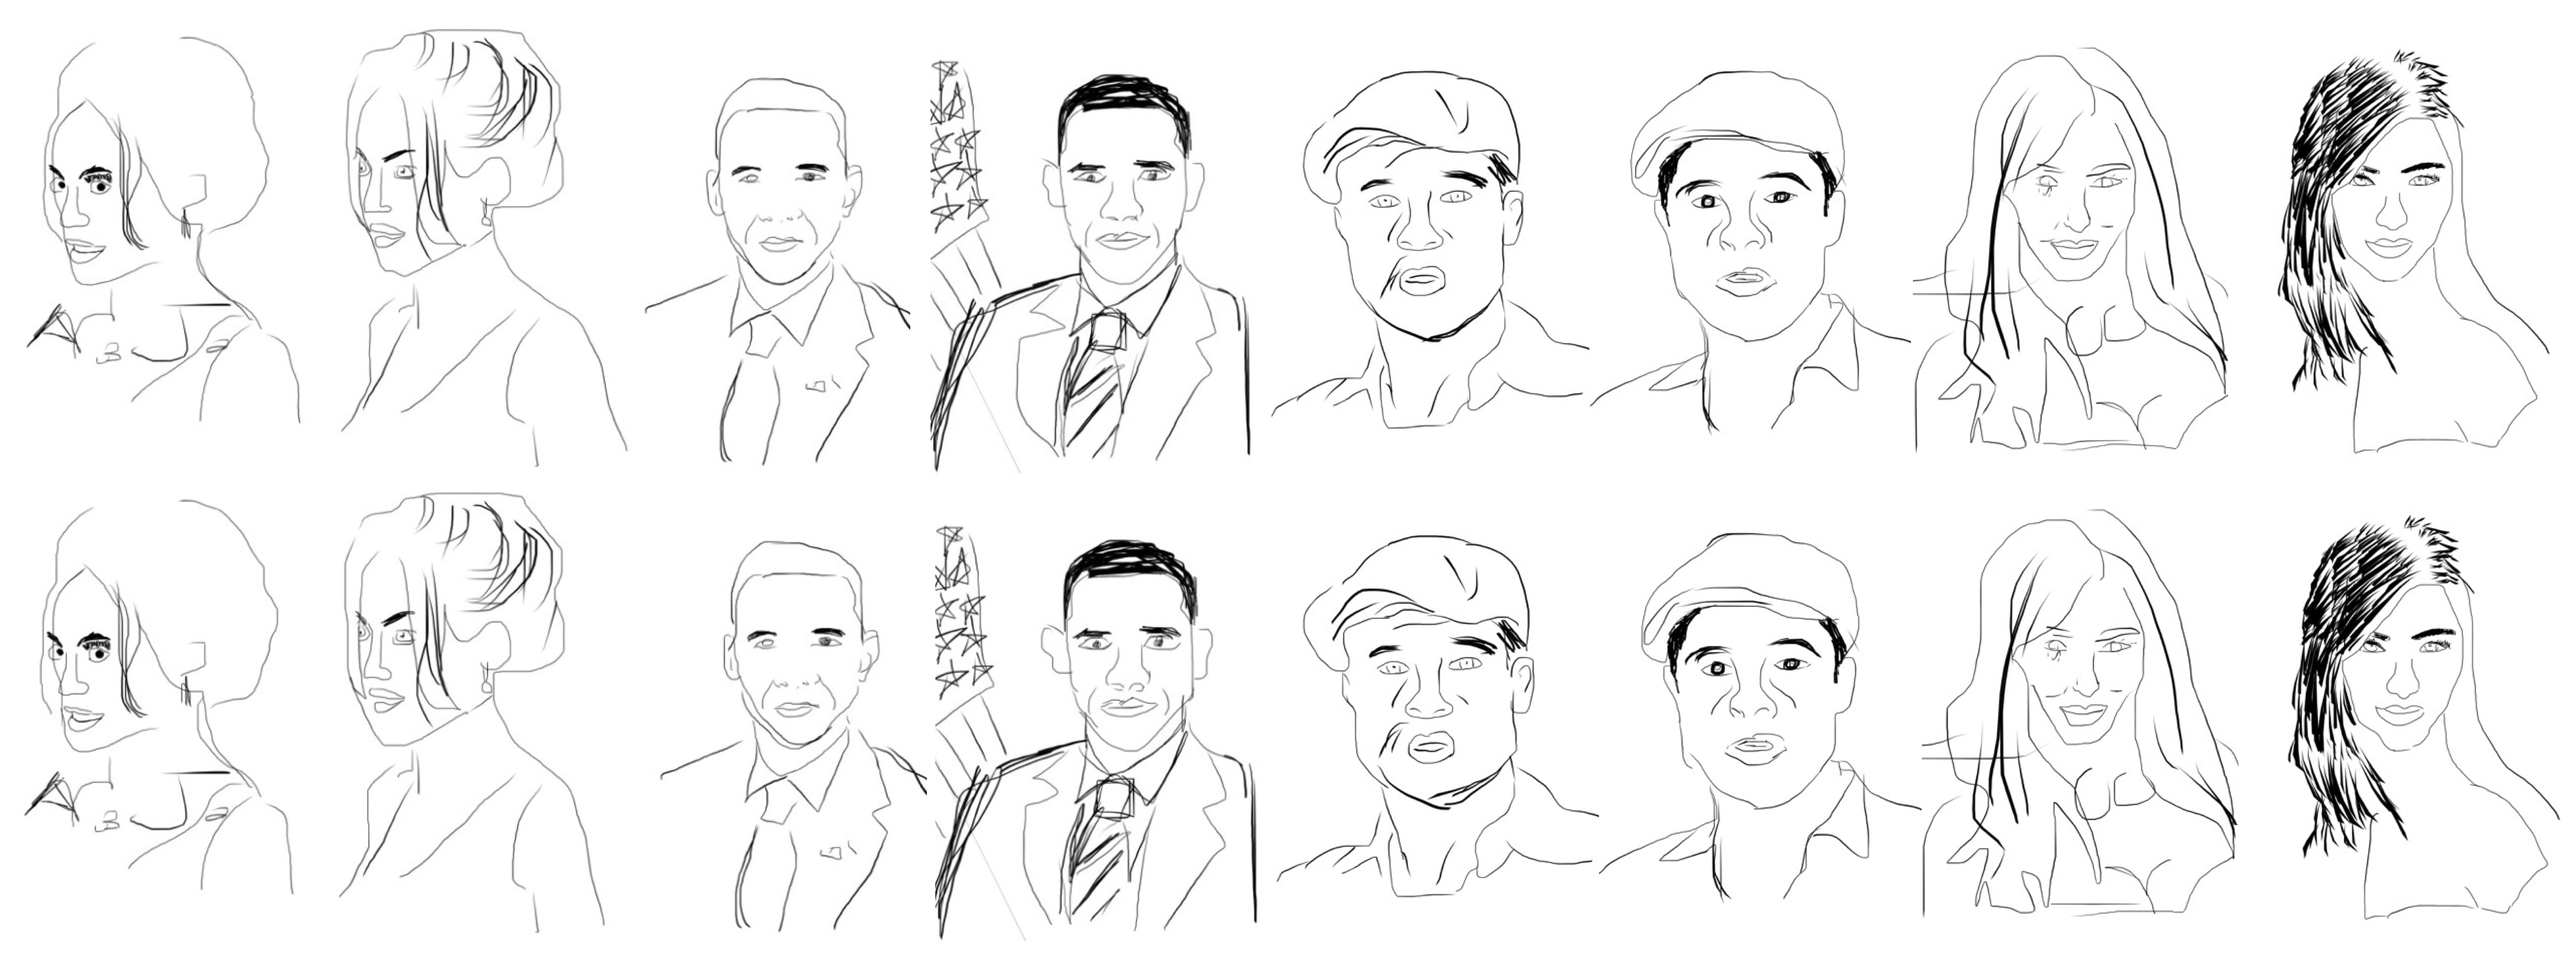
\includegraphics[width=7in]{./figures/ResultsAll_16.png}
\vspace{-0.35in}
  \caption{Celebrity drawings: original strokes (bottom rows) and after automatic adjustment to consensus (top rows). (Please see the supplementary files for more examples and also for an interface so you can flip between them.)}
\vspace{-0.25in}
  \label{fig:results}
\end{figure*}
